\documentclass[12pt, oneside]{article}
\usepackage{a4wide}
\usepackage{oldgerm}
\usepackage{amsmath}
\usepackage{amssymb}
\usepackage{amstext}
\setlength{\textheight}{8.875in} \setlength{\textwidth}{6.875in}
\setlength{\columnsep}{0.3125in} \setlength{\topmargin}{0in}
\setlength{\headheight}{0in} \setlength{\headsep}{0in}
\setlength{\parindent}{1pc} \setlength{\oddsidemargin}{-.304in}
\setlength{\evensidemargin}{-.304in}

\usepackage{graphicx}
\usepackage{caption}
\usepackage{subcaption}

\begin{document}
\setlength{\textheight}{8.5in}
\centering {\bf MTL 390 (Statistical Methods) }\\


\centering{\bf Minor Examination Assignment 1 Report}



\vskip 0.5cm

\noindent Name: Subhalingam D~~ ~~~  ~~~~~ ~~~~ ~~~~~~~~~~~~~~~~ Entry Number: 2018MT10770~~~~~~~~~~~



\vskip 0.5cm



\begin{enumerate}
	



\item	Descriptive Statistics
% student mark :: stem-leaf plot ::
%  inspired from https://web.iitd.ac.in/~nkurur/2012-13/IIsem/cyl110/index.html
%   
% 3-sigma analogy??

\textit{\textbf{Problem}}

The marks of a class of 50 students in a Quiz of 50 marks is given as a stem-leaf plot below. 
\\
\begin{align}
\centering
\begin{tabular}{r|l}
    0 &	0 1 1 1 2 2 2 3 4 4 4 5 6 6 6 7 7 8 9 9 \\
    1 &	0 2 2 3 5 6 6 7 7 8 9 \\
    2 &	3 4 5 6 9 \\
    3 &	0 2 2 3 5 7 8 9 \\
    4 &	0 2 3 4 5 5 \\
\end{tabular}
\end{align}

In this plot, the first column is known as \textit{stem}, which signifies the first digit of the mark, and the second column is known as leaf, whose values are placed to the right of the stem to get mark of one student. \textit{For example, data in the fourth row will be translated as 30, 32, 32 and so on.}

\begin{enumerate}
    \item Find the value of any three measures of central tendency?
    \item Find the standard deviation?
    \item Can the difficulty (easy/medium/difficult) of the quiz be obtained? Quantify it?
    \item Because of COVID19, all further exams are cancelled and the grading would be done based on the quiz marks. Students who are in the third quartile would get A grade in the course. Find the starting mark for A grade and number of students who would get A grade? 
    \item The teacher had promised to give bonus marks (+5) for those who attend all the classes. However, all students had 100\% attendance. How would mean and standard deviation get affected if 5 marks were added for all the students for attendance?
    % \item Is third quartile more scattered than the first quartile?
\end{enumerate}

\textit{\textbf{Solution}}

The stem-leaf plot can be translated to:
\\
\begin{align}
\centering
    \begin{tabular}{|l|}
    \hline
        0, 1, 1, 1, 2, 2, 2, 3, 4, 4, \\
        4, 5, 6, 6, 6, 7, 7, 8, 9, 9, \\
        10, 12, 12, 13, 15, 16, 16, 17, 17, 18, \\
        19, 23, 24, 25, 26, 29, 30, 32, 32, 33, \\
        35, 37, 38, 39, 40, 42, 43, 44, 45, 45  \\
           \hline
    \end{tabular}
\end{align}

\begin{enumerate}
    \item 
    \begin{enumerate}
        \item Mean $\mu$ = $\frac{\sum_{i=1}^{50}x_i}{50}$ = $\frac{914}{50}$ = $18.28$
        \item Median: The $25^{th}$ and $26^{th}$ mark is $15$ and $16$. So the median is $15.5$.
        \item Mode: 1,2,4,6 have the highest frequency (four students) and hence are the mode.
    \end{enumerate}
    
    \item If $\sigma^2 = \frac{ \sum_{i=1}^{50}(x_i - \mu)^2}{n}$, then the standard deviation is $\sigma$. Substituting the values, we get $\sigma^2 = \frac{10420.08}{50} = 208.4016$. Hence $\sigma = 14.4361214$.
    
    \item The number of students who have scored less than 25 is clearly higher than the number of students who have scored greater than 25. So the paper should have been difficult. 
    
    Skewness can be quantified using $\frac { \frac{ \sum_{i=1}^{50} (X-\mu) ^3}{n} }{\sigma^3}$. Upon substituting the values, we get $0.481008979$. It is positive because the number of students in the right is less than that in the left.
    
    \item Since there are 50 students, the third quartile would start somewhere from $38^{th}$ student (when sorted from low marks to high marks). The $38^{th}$ student has scored 32 marks and the $37^{th}$ student has scored 30 marks (<32 marks). Hence, the third quartile opens at $32$ marks and 13 students get A grade.
    
    \item The mean increases by 5 marks when 5 marks are added to each student. However, the standard deviation does not change as the distance between each observation and the mean remains the same.
    
\end{enumerate}


\item	Descriptive Statistics

\textit{\textbf{Problem}}

A teacher was having a look at the attendance database of a class of 30 students. He takes note of the time (in seconds) at which each student entered the class after it has started for a particular day. He gets the following data:
\begin{align}
\centering
\begin{tabular}{|l|}
    \hline
       10, 20, 30, 30, 30, 40, 40, 50, 50, 70,\\
       70, 70, 80, 80, 80, 100, 110, 130, 170, 220, \\
       250, 280, 310, 380, 410, 500, 530, 560, 590 \\
           \hline
    \end{tabular}
\end{align}

\begin{enumerate}
\item The teacher is interested to know the count of number of students in the class at each minute. More specifically, find the number of students who enter the class at every 1 minute interval starting from 0 (i.e. number of students who enter at [0-10s], [10s-20s], etc.). Make a frequency table and find the cummulative frequency?

\item Plot a histogram for the same interval size?
\item Plot less-than Ogive and more-than Ogive plots on the same graph?
\item From Ogive plots, find at which time interval the 15th student enters the class?
\end{enumerate}

\textit{\textbf{Solution}}

\begin{enumerate}
    \item The frequency distribution table is:

\begin{align}
\centering
    \begin{tabular}{|c|c|c|c|}
    \hline
    Class interval & Frequency & Cumm Frequency (less than) & Cumm Frequency (greater than) \\
    \hline
    0 - 60  &    9  & 9   & 30 \\
    60 - 120 &   8  & 17  & 21 \\
    120 -180 &   2  & 19  & 13 \\
    180 - 240 &  2  & 21  & 11 \\
    240 - 300 &  2  & 23  & 9 \\
    300 - 360 &  1  & 24  & 7 \\
    360 - 420 &  2  & 26  & 6 \\
    420 - 480 &  0  & 26  & 4 \\
    480 - 540 &  2  & 28  & 4 \\
    540 - 600 &  2  & 30  & 2 \\
        \hline
    \end{tabular}
\end{align}

\item The histogram is plotted in Figure \ref{fig:hist}

\begin{figure}[hbtp]
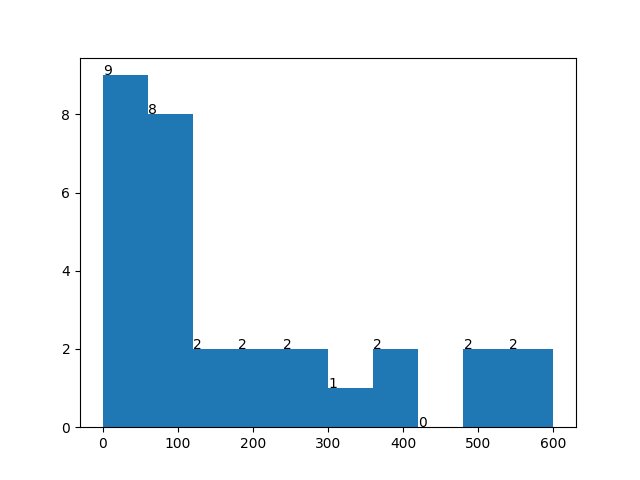
\includegraphics[width=\columnwidth]{Figure_1.png}
\caption{\label{fig:hist} Histogram for Q2}
\end{figure}

\item The Ogive graphs are (blue is for less-than Ogive and green is for more-than Ogive) plotted in Figure \ref{fig:ogive}.
\begin{figure}[hbtp]
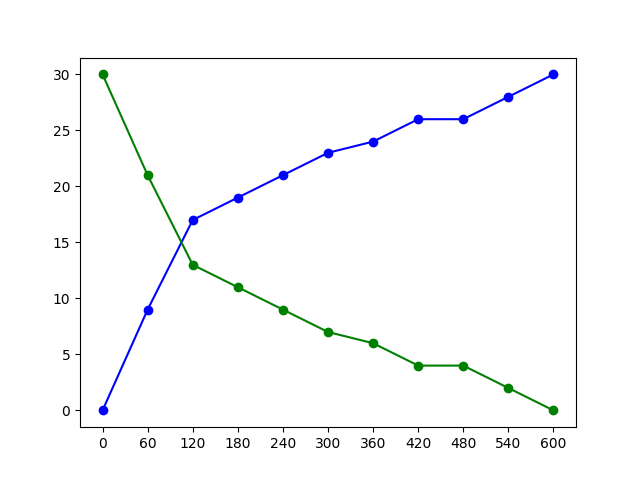
\includegraphics[width=\columnwidth]{Figure_2.png}
\caption{\label{fig:ogive} Ogive graphs for Q2}
\end{figure}

\item
The median can be obtained from the Ogive graph directly. The x-value of the point of intersection of less-than Ogive and more-than Ogive is the median. Hence, the 15th student enters between 1st and 2nd minute.

\end{enumerate}

\newpage

\item	Sampling Distributions

\textit{\textbf{Problem}}

You buy coffee regularly from Nescafe which is supposed to contain 200ml of coffee. However, because of crowd, the actual amount of coffee you get is normally distributed with mean 200ml and standard deviation 10ml. 

\begin{enumerate}
    \item You buy coffee from the shop regularly for 10 days (one each day) and measure the amount of coffee you get. What is the probability that the mean of these 10 numbers differs from required amount by more than 5ml?
   %  \item Find the probability that sample variance of the amount of coffee in these 10 days is greater than 5ml?
    \item Suppose they improve their services and the actual amount of coffee you get now is normally distributed with mean 200ml and standard deviation 5ml. Now, you buy coffee from the shop for 20 days (one per day) and get the mean of the measurements of the amount of coffee you actually get each day (simila to case (a)). What is the probability that this mean is greater than the mean obtained in case (a) by 5ml?

\end{enumerate}

\textit{\textbf{Solution}}


\begin{enumerate}
    \item We have samples $X_1,X_2,X_3,\dots,X_{10}$ each from $N(200,100)$ and all of these are independent (as the number of coffees available can be assumed to be large). If $\bar X= \frac{X_1+X_2+X_3+\dots+X_10}{10}$, then we know $\bar X \sim N(200,100/10)$. We want
    \[ P(|\bar X - 200|\ge5)=2P(\bar X - 200\ge5) =  2(1-0.943)=0.114\]
    
    % \item 
    
    \item Let $Y_1,Y_2,Y_3,\dots,Y_{20}$ be the new samples, each from $N(200,25)$, and all of these are independent. If $\bar Y= \frac{Y_1+Y_2+Y_3+\dots+Y_20}{20}$, then we know $\bar Y \sim N(200,25/20)$. 
    
    We need $P(\bar Y-\bar X>5)$. Since $\bar X$ and $\bar Y$ are independent, we have $Z = \bar Y - \bar X \sim N(200,1.25) - N(200,10) = N(0,11.25)$. Hence, 
    
    \[ P(Z>5) = 1- P(Z\le 5) = 1-0.932 = 0.068 \]
    
\end{enumerate}




\item	Sampling Distributions 

\textit{\textbf{Problem}}

Truncating values is one of the major steps while converting signals from analog-to-digital. Consider a device which truncates all the numbers after the decimal (i.e. 3.94 is converted 3). Such a device is fed with random values from $\mathbb{R}$ $n$ times, where $n$ is constant. Let $X_1,X_2,X_3,\dots,X_n$ denote the \textbf{truncation error} produced each time. Find the expected minimum and maximum value of truncation errors while the device was used $n$ times in the setup above. \textit{The truncation error when 3.94 is converted to 3 is 0.94.}

\textit{\textbf{Solution}}

Since the numbers fed into the device are random, the truncation error is Uniformly distributed from [0,1). Hence, $X_i \sim U(0,1) \forall i \in \{1,2,3,\dots,n\}$.

\begin{enumerate}
    \item 
    Let $Y \sim \min(X_1,X_2,...,X_n)$. The cdf of $Y$ is given as
    \[ F(y) = P(Y \le y) = 1 - P(Y > y) = 1 - P(\min(X_1,X_2,...,X_n) > y)\]
    However, $\min(X_1,X_2,...,X_n) > y$ means $X_i>y \forall i$. Due to independence, we have
    \[ F(y) = 1 -( P(X_1 > y)P(X_2 > y)\dots P(X_n > y) ) \]
    
    And $X_i \sim U(0,1)$, hence 
    \[ 
    F(y) = 
    \begin{cases}
        0 & y <0 \\
        1 - (1-y)^n & y \in [0,1] \\
        1 & y>1
    \end{cases}
    \]
    
    Differentiating to get $f(y)$,
    \[\begin{cases}
        n(1-y)^{n-1} & y \in [0,1] \\
        0 & \text{otherwise}
    \end{cases}
    \]
    
    \[E(Y) = \int_{-\infty}^\infty yf(y)dy = \frac{1}{n+1} \]
    
    Hence, the expected minimum truncation error is $\frac{1}{n+1}$.
    
    \item
    Let $X \sim \max(X_1,X_2,...,X_n)$. The cdf of $Z$ is given as
    \[ F(z) = P(Z \le z) = P(\max(X_1,X_2,...,X_n) \le z)\]
    However, $\max(X_1,X_2,...,X_n) \le z$ means $X_i\le z \forall i$. Due to independence, we have
    \[ F(z) = P(X_1 \le z)P(X_2 \le z)\dots P(X_n \le z)\]
    
    And $X_i \sim U(0,1)$, hence 
    \[ 
    F(z) = 
    \begin{cases}
        0 & z <0 \\
        z^n & z \in [0,1] \\
        1 & z>1
    \end{cases}
    \]
    
    Differentiating to get $f(z)$,
    \[\begin{cases}
        nz^{n-1} & z \in [0,1] \\
        0 & \text{otherwise}
    \end{cases}
    \]
    
    \[E(Z) = \int_{-\infty}^\infty zf(z)dz = \frac{n}{n+1} \]
    
    Hence, the expected maximum truncation error is $\frac{n}{n+1}$.
    
    
    

\end{enumerate}
    

\item	Point and Interval Estimations

\textit{\textbf{Problem}}

Let $X_1,X_2,X_3,\dots,X_n$ be $n(\in \mathbb{N})$ samples drawn independently from a Normal distribution with mean $\mu$ and variance $\sigma^2$. Let $\bar X_j = \frac{\sum_{i=1}^{j} X_i}{j}$ for $1 \le j \le n$. Further, denote $Z_j^2 = \frac{\sum_{i=1}^{j} (X_i - \bar X_j)^2}{j-1}$ for $1 \le j \le n$. \textit{Note that $\bar X_j$ and $Z_j^2$ are defined for given constant $j$}.
\begin{enumerate}
    \item Show that for each $j \in \{1,2,3,
    \dots,n\}$, $Z_j^2$ is an unbiased estimator of $\sigma^2$.
    \item Find the efficiency of $Z_j^2$ relative to $Z_k^2$ where $i,j \in \{1,2,3,\dots,n\}$ and $j\ne k$.
    \item From the result obtained from (b), which of the estimator $(Z_1^2,Z_2^2,\dots,Z_n^2)$ is most efficient?
\end{enumerate}

\textit{\textbf{Solution}}

For a given $j$, $\bar X_j = \frac{\sum_{i=1}^{j} X_i}{j}$ and since $X_i \sim N(\mu,\sigma^2)$, $\bar X_j \sim N(\mu,\sigma^2/j)$. 

Now, we show that $\frac{(j-1)Z_j^2}{\sigma^2} \sim \chi^2(j-1)$ (i.e., $\chi^2$ distribution with $j-1$ degrees of freedom).

% \[ Z_j^2 = \frac{\sum_{i=1}^{j} (X_i - \bar X_j)^2}{j-1} \]
% \[ \implies Z_j^2 \sim  \frac{\sum_{i=1}^{j} {(N(\mu,\sigma^2) - N(\mu,\sigma^2/j))^2}}{j-1} \]
% \[ \implies Z_j^2 \sim \frac{\sum_{i=1}^{j} {(N(0,\big(\frac{j-1)}{j}\big)\sigma^2) )^2}}{j-1} \]
% \[ \implies \frac{j(Z_j^2-0)}{(j-1)\sigma^2} \sim \frac{\sum_{i=1}^{j} {(N(0,1) )^2}}{j-1} \]

We know that $\sum_{i=1}^j (X_i - \mu)^2 = \sum_{i=1}^j (X_i - \bar{X_j})^2 + j(\bar{X_j} - \mu)^2$. By dividing by $\sigma^2$, we get:

\[ \sum_{i=1}^j \left(\frac{X_i - \mu}{\sigma}\right)^2 = \sum_{i=1}^j \left(\frac{X_i - \bar{X_j}}{\sigma}\right)^2 +  \left(\frac{\bar{X_j} - \mu}{\sigma/\sqrt{j}}\right)^2 \]

Using the following results:
\[Z \sim N(0,1) \implies Z^2 \sim \chi^2(1)\]
\[Z_i \sim \chi^2(1)\text{ and the }Z_i\text{ are independent }\implies\sum_{i=1}^n Z_i \sim \chi^2(n)\]

and,
\[ \sum_{i=1}^j \left(\frac{X_i - \bar{X_j}}{\sigma}\right)^2 = (j-1)\frac{Z_j^2}{\sigma^2} \]

Since $\bar{X_j}$ and $Z_j^2$ are independent. Using the moment generating function (where moment generating function for $\chi^2(n) = \frac{1}{(1-2t)^{n/2}}$). 

We finally get the moment generating function for $\frac{(j-1)Z_j^2}{\sigma^2}$ as 
\[ \dfrac{ \frac{1}{(1-2t)^{j/2}} }{ \frac{1}{(1-2t)^{1/2}} }= \frac{1}{(1-2t)^{(j-1)/2}}\]
which is the moment generating function for $\chi^2(j-1)$.



\begin{enumerate}
    \item For $Y \sim \chi^2$ distribution with $v$ degrees of freedom, $E(Y) = v$ and $Var(Y) = 2v$. Hence, \[E\bigg(\frac{(j-1)Z_j^2}{\sigma^2}\bigg) = (j-1)\] \[\implies \frac{(j-1)}{\sigma^2} E(Z_j^2) = j-1\] \[\implies E(Z_j^2) = \sigma^2\]
    Hence $Z_j^2$ is an unbiased estimator of $\sigma^2$.
    
    \item \[Var\bigg(\frac{(j-1)Z_j^2}{\sigma^2}\bigg) = 2(j-1)\] \[\implies \frac{(j-1)^2}{\sigma^4} Var(Z_j^2) = 2(j-1)\] \[\implies Var(Z_j^2) = \frac{2}{j-1}\sigma^4\]
    
    So relative efficiency of $Z^2_j$ and $Z^2_k$ is $\frac{k-1}{j-1}$.
    
    \item $Z_n$ is the most efficient 
    
\end{enumerate}


\item	Point and Interval Estimations

\textit{\textbf{Problem}}


Consider a study on genotypes for \textit{length of stem} of a peas plant. The genotypes can be represented as \textit{TT}, \textit{Tt} and \textit{tt}. The dominant gene (tall plants) are represented by \textit{T} while \textit{t} is used for the recessive gene (dwarf plants). The plants are tall in the first two cases and dwarf in the third case. The study was conducted on a sample of $500$ peas plants and the following data was obtained:

\begin{tabular}{l|l|l|l}
     \textbf{Genotype} & TT & Tt & tt  \\ \hline 
     \textbf{Number of samples} & 325 & 110 & 65 \\
\end{tabular}

It is known that genotypes \textit{TT}, \textit{Tt} and \textit{tt} occur with probabilities $(1 - \theta)^2$, $2\theta(1 - \theta)$ and $2\theta$ for some parameter $\theta$. \textit{Assume that the genotypes follow Multinomial distribution}.

\begin{enumerate}
    \item Find the Maximum Likelihood Estimator (MLE) of $\theta$?
    \item Find the asymptotic variance of the MLE obtained in part (a)?
    \item Find the large sample asymptotic distribution of the MLE obtained in part (a)?
    \item  Find an approximate 90\% confidence interval for $\theta$?
   % \item Does 90\% confidence mean that the probability $\theta$ is in the interval you found (in part (c)) is 90\%?
   \item Does 90\% confidence mean that the probability $\theta$ is in the interval you found (in part (d)) is 90\%?
\end{enumerate}

\textit{\textbf{Solution}}

Let $(X_1, X_2, X_3) \sim Multinomial(n = 500, p = ((1 - \theta)^2, 2\theta(1 - \theta), \theta^2$).

\begin{enumerate}
    \item Define the log likelihood
    
    \[ \ln L = \ln(f(x_1, x_2, x_3 ; p_1(\theta), p_2(\theta), p_3(\theta))) \]
    \[ \implies \ln L =  \ln \bigg( \frac{n!}{x_1!x_2!x_3!} p_1(\theta)^{x_1} p_2(\theta)^{x_2} p_3(\theta)^{x_3} \bigg) \]
    \[\implies \ln L = x_1 \ln((1 - \theta)^2) + x_2\ln(2\theta(1 - \theta)) +x_3\ln(\theta^2) + \text{(non-}\theta\text{ terms)} \]
    \[\implies \ln L = (2x_1 + x_2)\ln(1 - \theta) + (2x_3 + x_2)\ln(\theta) + \text{(non-}\theta\text{ terms)} \]
    
    Differentiating the log likelihood
    \[ \frac{\partial{L}}{\partial\theta} = -\frac{2x_1 + x_2}{1 - \theta} + \frac{2x_3 + x_2}{\theta}\]
    \[ \implies \hat \theta = \frac{2x_3 + x_2}{2x_1 + 2x_2 + 2x_3} =  \frac{2x_3 + x_2}{n} = \frac{2(65) + 110}{1000} = 0.24\]
    
    \item We know $Var(\theta) \to \frac{1}{E(-\frac{\partial^2 L}{\partial \theta^2})}$
    \[ \frac{\partial^2 L}{\partial \theta^2} = -\frac{2x_1 + x_2}{(1-\theta)^2} - \frac{2x_3 + x_2}{\theta^2} \]
    
    Since each $X_i \sim Binomial(n,p_i(\theta))$,
    \[ E(X_1) = np_1(\theta) = n(1-\theta)^2 \]
    \[ E(X_2) = np_2(\theta) = 2n\theta(1-\theta) \]
    \[ E(X_3) = np_3(\theta) = n(\theta^2) \]
    
    Hence,
    \[ E(-\frac{\partial^2 L}{\partial \theta^2}) = \frac{2n}{\theta(1-\theta)} = \frac{2(500)}{0.24(1-0.24)} = 5482.45\]
    
    Hence, the asymptotic variance is $1/5482.45 = 0.0001824$.
    
    \item The large sample asymptotic distribution of $\theta$ is $N(\theta, \frac{2n}{\theta(1-\theta)})$ by Central Limit Theorem.
    
    \item The interval is given as $[\bar\theta - z_{\alpha/2} \sqrt{Var(\bar \theta)} ,\bar\theta + z_{\alpha/2} \sqrt{Var(\bar \theta)}$. For 90\%, $\alpha=0.1$ and $z_{0.05} = 1.645$. $\sqrt{Var(\bar \theta)} \approx 0.0135$. 
    Hence, the approximate 90\% confidence interval for $\theta$ is $[0.24-0.0222,0.24+0.0222] = [0.2178, 0.2622]$
    
    \item No. 90\% confidence means that in 90\% of experiments the random interval will contain the true $\theta$ and not the probability that $\theta$ is in the given interval.
    
    
    
\end{enumerate}


\end{enumerate}

\end{document}
